% !TEX program = xelatex
% -------------------------------------------------------------
%  Clean CV template — Letter size (8.5 × 11 in)
% -------------------------------------------------------------
\documentclass[10pt,letterpaper]{article}

% ---------- ENCODING / FONTS ------------------------------------
\usepackage{fontspec}
\IfFontExistsTF{Roboto}
  {\setmainfont{Roboto}}
  {\setmainfont{Helvetica Neue}}

% ---------- GEOMETRY --------------------------------------------
\usepackage[
  letterpaper,
  left=0.55in,
  right=0.55in,
  top=0.8in,
  bottom=0.8in
]{geometry}

% ---------- COLOURS & GRAPHICS ----------------------------------
\usepackage[dvipsnames,svgnames,x11names]{xcolor}
\definecolor{primary}{HTML}{004A99}
\definecolor{accent}{HTML}{E6F4FF}

\usepackage{graphicx}
\usepackage{tikz}
\usetikzlibrary{calc}

% ---------- LAYOUT HELPERS --------------------------------------
\usepackage{paracol}
\columnratio{0.32}
\setlength{\columnsep}{0.25in}

\usepackage[most]{tcolorbox}
\tcbset{colback=accent, colframe=accent, boxrule=0pt, sharp corners}

\usepackage{enumitem}
\setlist[itemize]{noitemsep,topsep=0pt,leftmargin=*}

% ---------- HEADING STYLES --------------------------------------
\usepackage{sectsty}
\allsectionsfont{\color{primary}\bfseries\uppercase}
\subsectionfont{\color{primary}\bfseries}
\renewcommand{\thesection}{}

% ---------- UTILITIES -------------------------------------------
\newcommand{\cvName}[1]{\vspace*{0.3in}\textbf{\LARGE #1}}
\newcommand{\cvHeadline}[1]{\par\smallskip\textit{#1}}
\newcommand{\cvHr}{\vspace{0.5\baselineskip}\hrule height 1pt\color{primary}\vspace{0.7\baselineskip}}

%=================================================================
%                DOCUMENT
%=================================================================
\begin{document}

% -------------------- TWO–COLUMN LAYOUT -------------------------
\begin{paracol}{2}

% -------- LEFT SIDEBAR ------------------------------------------
\begin{leftcolumn}
\begin{center}
% --- Avatar -----------------------------------------------------
\begin{tikzpicture}
  \node[draw=primary,line width=1pt,circle,minimum width=1.6in,minimum height=1.6in,inner sep=0pt]  (photo) {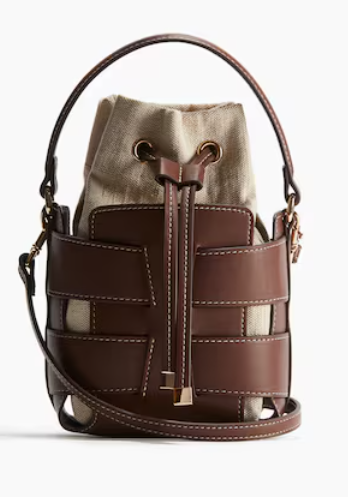
\includegraphics[width=1.6in,height=1.6in]{a1aeed49a5364e4b8d7cd0914f02256d.png}};
\end{tikzpicture}
\end{center}

% Vertical offset to align with summary start on right
\vspace{0.6in}

% --- Name & headline -------------------------------------------
\cvName{Pape FALL}
\cvHeadline{Data Scientist}

\cvHr

% --- Contact Information ---------------------------------------
\section*{Contact Information}
0753481453\\
papesalioufall2@gmail.com\\
12 Rue des Écoles, 75005 Paris, France

\cvHr

% --- Languages --------------------------------------------------
\section*{Languages}
\begin{itemize}
  \item Français (courant)
  \item Anglais (professionnel)
  \item Wolof (natif)
\end{itemize}

\cvHr

% --- Key Skills -------------------------------------------------
\section*{Key Skills}
\begin{itemize}
  \item Python, R, SQL
  \item Pandas, NumPy, Scikit-learn
  \item TensorFlow, Keras, PyTorch
  \item NLP (spaCy, Transformers)
  \item Data Viz : Matplotlib, Seaborn, Plotly
  \item Machine Learning \& Deep Learning
  \item MLOps (Docker, Git, CI/CD)
  \item Big Data : Spark, Hadoop
  \item Cloud : AWS, GCP
  \item Exploration & nettoyage de données
\end{itemize}

\cvHr

% --- Hobbies ----------------------------------------------------
\section*{Hobbies}
Football, Échecs, Concours de datavisualisation

\end{leftcolumn}

% -------- MAIN COLUMN ------------------------------------------
\begin{rightcolumn}

% --- Professional Summary --------------------------------------
\section*{Professional Summary}
Data Scientist passionné, spécialisé en modélisation prédictive, apprentissage profond et traitement du langage naturel.  
Solide expérience dans la mise en production de modèles ML et l’analyse de jeux de données complexes pour générer des insights business.  
Autonome, curieux et habitué à travailler dans un environnement agile, j’apporte une approche axée sur les résultats et la communication des données à des parties prenantes non techniques.

\vspace{1in}

% --- Work Experience -------------------------------------------
\section*{Work Experience}

% ----- Experience block 1 --------------------------------------
\begin{tcolorbox}
  \begin{minipage}[t]{0.48\linewidth}
    2022-05 --\\
    \textbf{Prepaya}\\
    \textit{Data Scientist — Paris, France}
    \begin{itemize}
      \item Construite un pipeline de traitement de données clients (10M+ enregistrements) réduisant de 30 \% le temps de préparation.
      \item Développé un modèle de prévision de churn (XGBoost) avec une précision de 87 \%, entraînant une baisse de 12 \% du taux d’attrition.
      \item Implémenté une API Flask pour la mise en production des modèles sur AWS Fargate, améliorant la latence de réponse \textless{} 200 ms.
      \item Mis en place des dashboards Power BI pour le suivi KPI qui ont aidé la direction à piloter la stratégie produit.
      \item Collaboration étroite avec les équipes produit et marketing dans un cadre agile (Scrum).
    \end{itemize}
  \end{minipage}\hfill
  \begin{minipage}[t]{0.48\linewidth}
    \raggedleft
    2023-08
  \end{minipage}
\end{tcolorbox}

\vspace{0.9in}

% --- Education --------------------------------------------------
\section*{Education}
\begin{tcolorbox}[colback=white,boxrule=1pt,colframe=primary]
  \begin{minipage}{0.47\linewidth}
    Master 2 — Data Science\\
    Sorbonne Université\\
    2022-2024
  \end{minipage}
\end{tcolorbox}

% --- Certifications --------------------------------------------
\section*{Certifications}
\begin{itemize}
  \item Jun 2023 — AWS Certified Machine Learning – Specialty (Amazon Web Services)
  \item Mar 2022 — Deep Learning Specialization (Coursera / DeepLearning.AI)
\end{itemize}

\end{rightcolumn}

\end{paracol}

\end{document}